\documentclass[a4paper, 11pt, twoside]{article}

\usepackage[brazilian]{babel} % Habilita o uso de portugues brasileiro
\usepackage{lmodern}
\usepackage[T1]{fontenc}

\usepackage[square, numbers, comma, sort&compress]{natbib} 
\usepackage{verbatim}  % Comment environment
\usepackage[margin=2.5cm]{geometry}
\usepackage{amsmath}	% Matrices
\usepackage{subfig}
\usepackage{graphicx}
\usepackage{url}
\usepackage{hyperref}
\usepackage{xcolor}
\usepackage{algorithm}
\usepackage{algpseudocode}
\usepackage[retainorgcmds]{IEEEtrantools}

\usepackage[margin=10pt, font=small, labelfont=bf]{caption}  % customise caption style

% from https://www.overleaf.com/learn/latex/code_listing
\usepackage{upquote, textcomp}  % required for upticks in listings env
\usepackage{listings}
\definecolor{codegreen}{rgb}{0, 0.6, 0}
\definecolor{codegray}{rgb}{0.5, 0.5, 0.5}
\definecolor{codepurple}{rgb}{0.58, 0, 0.82}
\definecolor{backcolour}{rgb}{0.95, 0.95, 0.95}

\lstset{backgroundcolor=\color{backcolour},   
	commentstyle=\color{codegreen},
	keywordstyle=\color{magenta},
	numberstyle=\tiny\color{codegray},
	stringstyle=\color{codepurple},
	basicstyle=\ttfamily\footnotesize,
	breakatwhitespace=false,         
	breaklines=true,                 
	captionpos=b,                    
	keepspaces=true,                                 
	showspaces=false,                
	showstringspaces=false,
	showtabs=false,                  
	tabsize=4,
	upquote=true,
	frame=single,
	language=Python
}

\hypersetup{urlcolor=blue, colorlinks=true, linkcolor=blue, citecolor=blue}  % Colours hyperlinks in blue, but this can be distracting if there are many links.

% Use double bar for vector norm
\providecommand{\norm}[1]{\lVert#1\rVert}

% "upright" 'd' for integrals
\newcommand{\ud}{\,\mathrm{d}}

% "AmT" in typewriter font (use as "\AmT{}" to avoid spacing issues)
\newcommand{\AmT}{\texttt{AmT}}



\author{Fabio Casagrande Hirono \\ \texttt{fchirono@gmail.com}}
\title{\texttt{amiet\_tools}: um pacote em Python para predição de ruído de interação turbulência-aerofólio\\\textcolor{red}{EM CONSTRUÇÃO}}
\date{Fevereiro 2021}

\begin{document}
\maketitle

\begin{abstract}
	O pacote \verb|amiet_tools| (\AmT{}), escrito em linguagem Python, é uma implementação do modelo analítico de Amiet \cite{Amiet75} para predição de ruído de interação turbulência-aerofólio, com extensões. As funções permitem o cálculo da flutuação de pressão na superfície do aerofólio (i.e. a distribuição da fonte acústica) gerado em resposta à turbulência incidente, e do campo acústico radiado por esta interação. A turbulência incidente pode ser uma única rajada senoidal, ou uma soma incoerente de rajadas com amplitudes definidas por um espectro energético. Outras funções includem a modelagem de efeitos de convecção e refração na propagação sonora para modelar medições acústicas realizadas em túneis de vento abertos ou fechados. Uma publicação de referência está disponível \cite{Casagrande_etal2020}, e o pacote pode ser encontrado através do link \url{https://github.com/fchirono/amiet_tools}.
\end{abstract}

% *-*-*-*-*-*-*-*-*-*-*-*-*-*-*-*-*-*-*-*-*-*-*-*-*-*-*-*-*-*-*-*-*-*-
\section{Introdução}

\subsection{Contexto}

O ruído gerado pela interação entre um escoamento turbulento e uma superfície sólida, tal como um aerofólio, é uma das principais fontes de ruído banda larga na indústria de aviação moderna. Apesar dos mecanismos físicos fundamentais desta fonte de ruído estarem bem estabelecidos, métodos eficientes para redução de ruído de interação turbulência-aerofólio ainda são objeto de estudos e pesquisas. Devido ao seu baixo custo computacional, modelos analíticos são frequentemente adotados para analisar os comportamentos físicos fundamentais e escalas do problema. Entre os modelos analíticos mais populares para predição de ruído de aerofólio, o modelo de Amiet \cite{Amiet75} para um aerofólio do tipo placa plana em campo livre é frequentemente considerado um dos mais importantes devido a sua simplicidade formal e extensibilidade.

Em resumo, o modelo de Amiet decompõe um escoamento turbulento em uma soma de Fourier, onde cada componente constitui uma ``rajada'' turbulenta senoidal, e calcula a flutuação de pressão --- também denominada ``salto de pressão'' --- sobre a superfície do aerofólio em resposta à interação com cada rajada. Seguindo a analogia acústica de Ffowcs Williams e Hawkings, a radiação acústica pode ser calculada usando uma distribuição de fontes tipo dipolo pontual sobre a superfície do aerofólio, cuja amplitude é dada pelo salto de pressão. O campo acústico radiado é então calculado através de uma integral de radiação, levando-se em conta os efeitos de convecção e/ou refração do som na propagação entre a fonte e o(s) observador(es).

Ao assumir que o aerofólio possui envergadura infinita (uma aproximação teórica para aerofólios de alta razão de aspecto, ou para envergaduras muito maiores que o comprimento de onda acústico), pode-se mostrar que uma única rajada senoidal será responsável por todo o ruído recebido por um observador distante. A expressão resultante desta simplificação relaciona a densidade espectral de potência (\emph{power spectral density} -- PSD) do ruído visto pelo observador diretamente às propriedades do escoamento turbulento e à geometria do aerofólio, evitando assim o cálculo da distribuição de fonte acústica sobre a superfície do aerofólio e da integral de radiação completa. Esta forma simplificada do modelo de Amiet é a mais popular, e é geralmente suficiente para se obter as tendências gerais do ruído radiado. 

Porém, tais aproximações podem ser simplórias demais para problemas mais avançados, tais como o cálculo explícito do campo acústico próximo ao aerofólio, ou a inclusão de efeitos de envergadura finita ou de rajadas múltiplas. Sob estas condições, o modelo de Amiet requer o cálculo separado da distribuição de fontes e da integral de radiação, realizados de forma probabilística através das funções densidade espectral cruzada (\emph{cross-power spectral density} -- CSD), aumentando significativamente a complexidade das operações necessárias. Neste caso, é interessante buscar uma implementação de referência do modelo de Amiet completo, permitindo que os pesquisadores possam obter resultados confiáveis rapidamente e não perder tempo com detalhes de implementação.

Este documento busca introduzir o pacote \verb|amiet_tools| (abreviado por ``\AmT{}''), uma implementação de referência do modelo de Amiet completo para ruído de interação turbulência-aerofólio \cite{Casagrande_etal2020}, e explicar o seu uso. O pacote \AmT{} é desenvolvido em linguagem Python e disponibilizado com uma licença de código aberto, permitindo a sua distribuição, modificação e uso por diversos usuários em múltiplos sistemas operacionais. O pacote encontra-se hospedado na plataforma GitHub através do link:

\begin{itemize}
	\item \url{https://github.com/fchirono/amiet_tools} .
\end{itemize}


\subsection{Referências teóricas recomendadas}

Este documento não busca explicar completamente a teoria por trás do modelo de Amiet. Para mais detalhes e informações sobre modelo analítico completo, recomendamos que o leitor consulte outras referências na literatura, entre as quais recomendamos:

\begin{itemize}
	\item R. Amiet, ``\emph{Acoustic radiation from an airfoil in a turbulent stream}'', Journal of Sound and Vibration, Vol. 41, No. 4:407–420, 1975 \cite{Amiet75};
	
	\item G. Reboul, ``\emph{Modélisation du bruit à large bande de soufflante de turboréacteur}'', PhD Thesis, Laboratoire de Mécanique des Fluides et d’Acoustique -- École Centrale de Lyon, Lyon -- France, 2010 \cite{Reboul10};
	
	\item M. Roger, ``\emph{Broadband noise from lifting surfaces: Analytical modeling and experimental validation}'', in: R. Camussi (Ed.), ``\emph{Noise Sources in Turbulent Shear Flows: Fundamentals and Applications}'', Springer-Verlag, 2013 \cite{Roger13};
	
	\item L. de Santana, ``\emph{Semi-analytical methodologies for airfoil noise prediction}'', PhD Thesis, Faculty of Engineering Sciences -- Katholieke Universiteit Leuven, Leuven, Belgium, 2015 \cite{deSantana2015};
	
	\item F. Casagrande Hirono, ``\emph{Far-Field Microphone Array Techniques for Acoustic Characterisation of Aerofoils}'', PhD Thesis, Institute of Sound and Vibration Research, University of Southampton, Southampton -- UK, 2018 \cite{Casagrande18}.
\end{itemize}

% *-*-*-*-*-*-*-*-*-*-*-*-*-*-*-*-*-*-*-*-*-*-*-*-*-*-*-*-*-*-*-*-*-*-
\clearpage
\newpage
\section{O modelo de Amiet}

Esta seção busca descrever os principais conceitos por trás do modelo de Amiet. O modelo estima as características do campo acústico radiado como função das condições experimentais do problema: as propriedades do escoamento turbulento, a geometria do aerofólio, e a localização dos observadores no campo acústico. Todos os cálculos são realizados no domínio da frequência (isto é, assume-se que todas as variáveis acústicas oscilam harmonicamente), e a cada frequência de interesse são realizadas três etapas:

\begin{enumerate}
	\item Decomposição do escoamento turbulento em múltiplas rajadas senoidais, cada uma caracterizada por seu número de onda lateral $k_\psi$;
	\item Cálculo do ``salto'' de pressão $\Delta p$ sobre o aerofólio em resposta a cada rajada turbulenta;
	\item Cálculo do campo acústico através de uma integral de radiação, levando em consideração efeitos de convecção e/ou refração na propagação do som.
\end{enumerate}


%Ao considerarmos a interação do aerofólio com uma rajada única, tanto a distribuição de pressão sobre o aerofólio quanto o ruído radiado a partir desta são determinísticos, isto é, coerentes: nesse caso, haverá interferência construtiva e destrutiva entre os sons gerados por cada ponto. Porém, as múltiplas rajadas que compõem um escoamento turbulento são incoerentes entre si, e a soma das contribuições de diferentes rajadas será um processo estocástico. Portanto, o ruído gerado também será de natureza estocástica, e deve ser analizado de forma probabilística através da função densidade espectral cruzada (\emph{cross spectral density} - CSD).

As condições experimentais do problema estão indicadas na Figura \ref{fig:experimental_setup}: um aerofólio do tipo placa plana retangular, de espessura infinitesimal, está imerso em um escoamento turbulento subsônico de velocidade $U_x$ e número Mach $M_x = U_x/c_0$ na direção $+x$. O aerofólio possui corda $c=2b$ e envergadura $L=2d$ (e portanto, razão de aspecto $L/c$), e a origem do sistema de coordenadas é posicionada no centro do aerofólio, com o eixo $+z$ perpendicular ao aerofólio (apontando ``fora da página'' na Fig. \ref{fig:experimental_setup}). Pontos no espaço ao redor do aerofólio são indicados por um vetor $\mathbf{r}=(x, y, z)$, e pontos na superfície do aerofólio são indicados com um caractere subescrito ``$_s$'', da forma $\mathbf{r}_s = (x_s, y_s, z_s)$. O aerofólio encontra-se no plano $z_s = 0$. A análise aqui apresentada encontra-se no domínio da frequência angular $\omega = 2 \pi f$, e a dependência temporal implícita é da forma $e^{+j \omega t}$.

\begin{figure}[htbp]
	\centering
	\includegraphics[width=0.6\textwidth]{../figures/Oblique_Gust_aerofoil.pdf}
	\caption{Diagrama das condições experimentais}
	\label{fig:experimental_setup}
\end{figure}

\subsection{Interação com uma rajada única}

\subsubsection{Flutuação de pressão sobre o aerofólio}

Um espectro contínuo de rajadas turbulentas senoidais ``congeladas'' move-se no plano $z=0$ com velocidade de convecção $U_x$, e cada rajada é definida por um par de números de onda hidrodinâmicos (isto é, vorticais) longitudinal e lateral $(k_\chi, k_\psi)$. Uma rajada única representa uma perturbação de velocidade vertical, conforme indicado na Figura \ref{fig:gust_airfoil_2D}, e é da forma

\begin{equation}
w(x, y, \omega) = \hat{w}_0(\kappa_\chi, k_\psi) e^{-j\kappa_\chi x} e^{-j k_\psi y },
\end{equation}

\noindent onde $\kappa_\chi = \omega/U_x$ é o número de onda longitudinal da rajada, associado unicamente à frequência $\omega$ do ruído radiado, e $\hat{w}_0$ é a amplitude desta rajada. %Note que o número de onda lateral $k_\psi$ pode assumir qualquer valor real em qualquer frequência, e portanto em problemas envolvendo múltiplas rajadas será necessário integrar a contribuição dos diferentes números de onda laterais a cada frequência.

\begin{figure}[htbp]
	\centering
	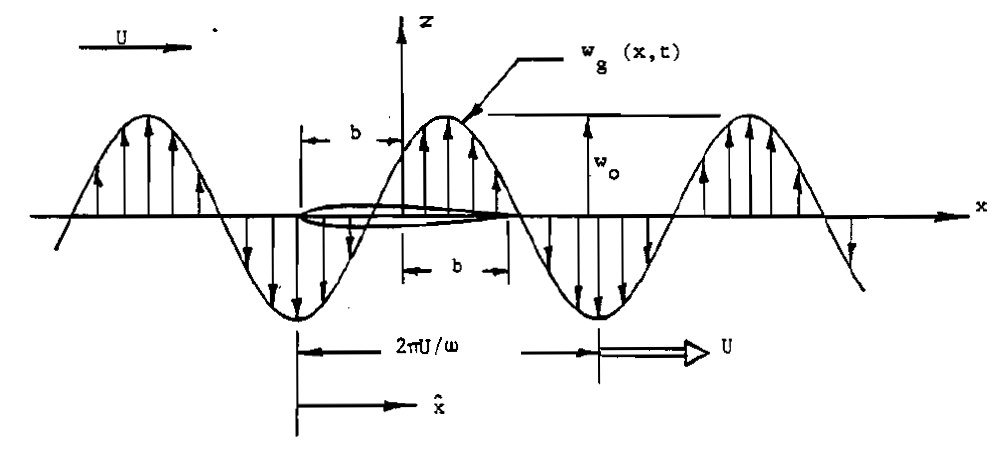
\includegraphics[width=0.8\textwidth]{../figures/gust_ProfGil_ITA_aula06.jpg}
	\caption{Diagrama 2D indicando uma perturbação de velocidade vertical $w(x, t)$ (``rajada'' turbulenta) interagindo com um aerofólio. [Figura reproduzida a partir dos materiais da disciplina \emph{AA-220 -- Aerodinâmica Não Estacionária}, Prof. Dr. Roberto Gil Annes da Silva, ITA, Brasil -- \url{http://www.aer.ita.br/~gil/disciplinas/aa-220/aa2206.pdf}].}
	\label{fig:gust_airfoil_2D}
\end{figure}


Em resposta à incidência de uma única rajada turbulenta, haverá uma flutuação na pressão sobre a superfície do aerofólio, denominada aqui de ``salto'' de pressão $\Delta p$. Este salto de pressão será da forma

\begin{equation}
\Delta p(x_s, y_s, \omega) =  2 \pi \rho_0 \hat{w}_0(\kappa_\chi, k_\psi) \ g(x_s, \kappa_\chi, k_\psi) e^{-j k_\psi y_s},
\label{eq:DeltaP_SingleGust}
\end{equation}

\noindent onde $g$ é o salto de pressão não-dimensional sobre a corda $x_s$ devido a uma rajada $(\kappa_\chi, k_\psi)$. Note que a distribuição da flutuação de pressão ao longo da envergadura apresenta o mesmo comportamento lateral da rajada turbulenta, dado por $e^{-j k_\psi y_s}$.

O salto de pressão não dimensional $g(x_s, \kappa_\chi, k_\psi)$, também chamado de função de resposta do aerofólio, associa a distribuição da flutuação de pressão $\Delta p$ sobre a corda do aerofólio aos números de onda $(\kappa_\chi, k_\psi)$ da rajada turbulenta que o gerou. Alguns exemplos de $g$ para diferentes valores de $k_\psi$ estão plotados na Figura \ref{fig:Abs_gLE_kc50}. Esta função apresenta uma singularidade no bordo de ataque, e tende a zero no bordo de fuga devido à condição de Kutta.


\begin{figure}
	\centering
	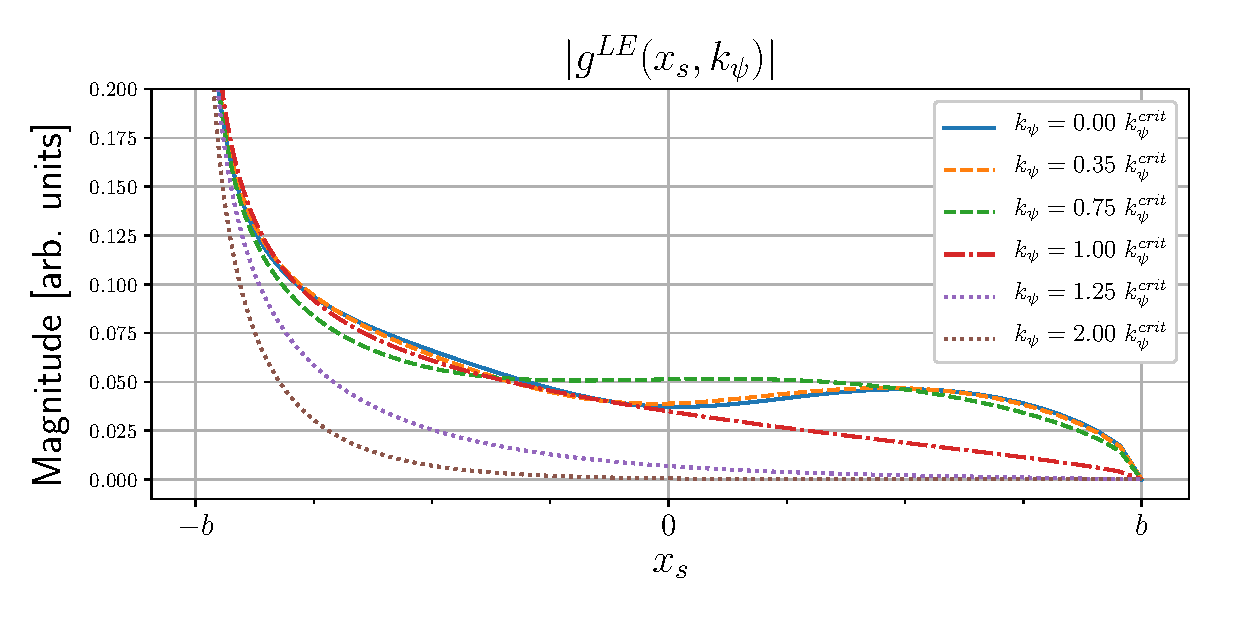
\includegraphics[width=0.85\textwidth]{../figures/Abs_gLE_ky_kc50.eps}
	\caption{Magnitude da função de resposta do aerofólio $g(x_s)$ para diferentes rajadas turbulentas, em unidades arbitrárias. A linha sólida indica uma rajada de incidência paralela (supercrítica); as linhas tracejadas indicam rajadas supercríticas de incidência oblíqua; a linha traço e ponto indica uma rajada crítica; e as linhas pontilhadas indicam rajadas subcríticas; $k_0 c = 5$, $M_x \approx 0.17$. [Figura adaptada de \citet{Roger13}]}
	\label{fig:Abs_gLE_kc50}
\end{figure}

\subsubsection{Radiação acústica}

Segundo a analogia de Ffowcs Williams e Hawkings, o ruído gerado por esta interação pode ser calculado usando uma distribuição equivalente de fontes pontuais tipo dipolo, com a flutuação de pressão $\Delta p$ sobre o aerofólio exercendo o papel de amplitude dos dipolos equivalentes. Analiticamente, a pressão acústica $p(\mathbf{r}, \omega)$ recebida por um observador no ponto $\mathbf{r} = (x, y, z)$ é dada por

\begin{equation}
	p(\mathbf{r}, \omega) = \int_{-d}^{+d} \int_{-b}^{+b} \Delta p(\mathbf{r}_s, \omega) \frac{\partial }{\partial z_s} G_{U_x}(\mathbf{r} | \mathbf{r}_s, \omega) \ud x_s \ud y_s,
	\label{eq:ac_radiation_single_gust}
\end{equation}

\noindent onde o termo $\partial G_{U_x}(\mathbf{r} | \mathbf{r}_s, \omega) / \partial z_s$ representa a função de transferência de uma fonte tipo dipolo localizada em $\mathbf{r}_s$ e o observador em $\mathbf{r}$, onde ambos estão imersos em um escoamento uniforme de velocidade $U_x$. Esta função de transferência é dada por

\begin{equation}
	\frac{\partial}{\partial z_s} G_{U_x} (\mathbf{r} | \mathbf{r}_s, \omega) = \left(jk_0 + \frac{1}{\overline{r}} \right) \frac{\left(\overline{z}-\overline{z}_s \right)}{\beta \overline{r}}  \frac{e^{-j k_0 \overline{r}}}{4 \pi \beta^2 \overline{r}} e^{j k_0 M_x \left( \overline{\overline{x}} - \overline{\overline{x}}_s \right)},
	\label{eq:ConvDipole}
\end{equation}

\noindent onde a sobrelinha representa uma transformação de variáveis do tipo Prandtl-Glauert para descrever os efeitos do escoamento no campo acústico \cite{Chapman00}:

\begin{equation}
	\overline{\mathbf{r}} = \left( \overline{\overline{x}}, \overline{y}, \overline{z} \right) = \left( \frac{x}{\beta^2}, \frac{y}{\beta}, \frac{z}{\beta} \right), \quad \overline{r} = \norm{\overline{\mathbf{r}} - \overline{\mathbf{r}}_s}, \quad \beta = \sqrt{1-M_x^2}.
	\label{eq:ChapmanTransformedVariables}
\end{equation}

Se as condições experimentais adotam um túnel de vento aberto, a função de transferência dada pela Eq. \ref{eq:ConvDipole} pode ser modificada para incluir efeitos de refração das ondas acústicas na camada cisalhante gerada entre o escoamento gerado pelo túnel e o ar estacionário ao redor deste. Mais detalhes podem ser encontrados nas referências \cite{Casagrande18, Casagrande_etal2020}, por exemplo.

Conforme descrito acima, a flutuação de pressão $\Delta p$ em resposta a uma única rajada turbulenta será completamente coerente --- isto é, todos os pontos na superfície do aerofólio flutuarão na mesma frequência e perfeitamente em fase, de forma estatisticamente \emph{dependente}, e o campo acústico $p$ gerado por esta interação exibirá efeitos de interferência construtiva e destrutiva entre as diferentes regiões do aerofólio.


\subsubsection{Implementação numérica}
\label{sec:NumericalImplementation_SingleGust}

Para calcular numericamente a radiação acústica recebida por uma série de observadores em $M$ posições $\mathbf{r}_m$, $m \in [1, \ldots, M]$, adotamos uma formulação matricial do problema. Primeiramente, definimos um vetor $\mathbf{p} = [p(\mathbf{r}_1), p(\mathbf{r}_2), \ldots, p(\mathbf{r}_M)]^T$ contendo as pressões acústicas nas $M$ posições de interesse. Este vetor de pressões acústicas está relacionado a um vetor contendo $N$ ``amplitudes de fonte'' discretizadas $\mathbf{q} = [q_1, \ldots, q_N]$ e a uma matriz de funções de transferências $\mathbf{G}$ da forma

\begin{IEEEeqnarray}{rCl}
	\mathbf{p} & = & \begin{bmatrix}
		|				&	|				&			& | \\
		\mathbf{g}_1	&	\mathbf{g}_2	&	\ldots 	& \mathbf{g}_N \\
		|				&	|				&			& | \\
	\end{bmatrix}
	\begin{bmatrix}
		q_1 \\
		q_2 \\
		\vdots \\
		q_N
	\end{bmatrix} \\
	& = & \mathbf{G} \mathbf{q}.
	\label{eq:ac_radiation_narrowband_discrete}
\end{IEEEeqnarray}

A matriz $\mathbf{G}$ contém as $M \times N$ funções de transferência ligando as $N$ fontes discretizadas à pressão acústica observada em $M$ pontos. Para popular a matriz $\mathbf{G}$, pode-se adotar a Equação \ref{eq:ConvDipole} para observadores imersos em um escoamento uniforme, ou ainda versões modificadas para incluir efeitos de refração acústica na camada cisalhante.

Para definir o vetor de fontes $\mathbf{q}$, a superfície do aerofólio é discretizada em $N$ pontos $\mathbf{r}_{s,n}$, $n \in [1, \ldots, N]$. O pacote \AmT{} usa uma discretização não uniforme na direção da corda com $N_x$ pontos, e uma discretização uniforme na direção da envergadura com $N_y$ pontos, de forma que $N = N_x \cdot N_y$. Assim, cada amostra $\mathbf{r}_{s,n} = (x_{s,n}, y_{s,n})$ na superfície do aerofólio possuirá uma ``área'' equivalente $dx[n] \cdot dy[n]$, onde $dx$ varia em funcão de $n$ e $dy$ é constante. 

Para que a Equação \ref{eq:ac_radiation_narrowband_discrete} seja uma aproximação discreta da Equação \ref{eq:ac_radiation_single_gust}, o vetor de fontes $\mathbf{q}$ é construído de forma que o seu $n$-ésimo elemento $q_n$ contenha a flutuação de pressão $\Delta p(x_{s,n}, y_{s,n})$ amostrada no ponto $\mathbf{r}_{s,n}$ multiplicado pela ``área'' equivalente $dx[n] \cdot dy[n]$ desta mesma amostra:

\begin{equation}
	\mathbf{q} =
	\begin{bmatrix}
		\Delta p(x_{s,1}, y_{s,1}) \cdot dx[1] \cdot dy[1] \\
		\Delta p(x_{s,2}, y_{s,2}) \cdot dx[2] \cdot dy[2]  \\
		\vdots \\
		\Delta p(x_{s,N}, y_{s,N}) \cdot dx[N] \cdot dy[N]
	\end{bmatrix}.
	\label{eq:sourceVector_q}
\end{equation}

A discretização da superfície do aerofólio é discutido em mais detalhes na Seção \ref{sec:SingleGustInteraction}.

\subsection{Interação com múltiplas rajadas}

Um escoamento turbulento isotrópico é um processo estocástico, e pode ser decomposto em um espectro contínuo de rajadas turbulentas incoerentes --- isto é, estatisticamente \emph{independentes} entre si. Portanto, a soma das contribuições de diferentes rajadas deve ser realizada de forma probabilística através das funções densidade espectral cruzada (CSD) da flutuação de pressão $S_{\Delta p \Delta p'}$ e do campo acústico $S_{pp'}$, que capturam as relações de magnitude e fase média destas grandezas entre dois pontos arbitrários.

A densidade espectral cruzada da flutuação de pressão $S_{\Delta p \Delta p'} (x_s, x_s', y_s, y_s', \omega)$ entre dois pontos $(x_s,y_s)$ e $(x_s', y_s')$ na superfície do aerofólio é dada por

\vspace{-15pt}
\begin{IEEEeqnarray}{rCl}
	S_{\Delta p \Delta p'} (x_s, x_s', y_s, y_s', \omega) & = & \lim_{T \rightarrow \infty} \left[ \frac{\pi}{T} \mathrm{E} \left\{ \Delta p(x_s, y_s, \omega) \Delta p^*(x_s', y_s', \omega) \right\} \right] \\
	& = &  (2 \pi \rho_0)^2 U_x \int_{-\infty}^{+\infty} \Phi_{ww}(\kappa_\chi, k_\psi) g(x_s, \kappa_\chi, k_\psi) g^*(x_s', \kappa_\chi, k_\psi) e^{-j k_\psi (y_s - y_s')} \ud k_\psi, \IEEEeqnarraynumspace
	\label{eq:SurfPressure_CSD}
\end{IEEEeqnarray}

\noindent onde $\Phi_{ww}(k_\chi, k_\psi)$ é a densidade espectral de número de onda da turbulência incidente. Aqui usamos a relação de ortogonalidade entre os diferentes números de onda em um escoamento turbulento homgêneo \cite{Amiet75}, dada por

\begin{equation}
	\lim_{T \rightarrow \infty} \left[ \frac{\pi}{T} \mathrm{E} \left\{ w(\kappa_\chi, k_\psi) w^*(\kappa_\chi, k_\psi') \right\} \right] = U_x \delta(k_\psi - k_\psi') \Phi_{ww}(\kappa_\chi, k_\psi).
	\label{eq:gust_orthogonality}
\end{equation}

Observe que a CSD apresentada na Equação \ref{eq:SurfPressure_CSD} é obtida a partir da integração sobre todos os números de onda laterais $k_\psi$ da turbulência, e portanto incorpora os efeitos de múltiplas rajadas.

Por sua vez, a densidade espectral cruzada do campo acústico $S_{pp'}(\mathbf{r}, \mathbf{r}', \omega)$ entre dois observadores em $\mathbf{r}$ e $\mathbf{r}'$ é dada por

\begin{IEEEeqnarray}{rCl}
	S_{pp'}(\mathbf{r}, \mathbf{r}', \omega) & = & \lim_{T \rightarrow \infty} \left[ \frac{\pi}{T} \mathrm{E} \left\{ p(\mathbf{r}, \omega) p^* (\mathbf{r}', \omega) \right\} \right] \\
	& = & \int_{-d}^{+d} \int_{-b}^{+b} \int_{-d}^{+d} \int_{-b}^{+b} S_{\Delta p \Delta p'} (\mathbf{r}_s, \mathbf{r}_s', \omega) \frac{\partial}{\partial z_s} G_{U_x} (\mathbf{r} | \mathbf{r}_s, \omega) \frac{\partial}{\partial z_s'} G^{*}_{U_x}(\mathbf{r}' | \mathbf{r}_s', \omega) \ud x_s \ud y_s \ud x_s' \ud y_s'. \IEEEeqnarraynumspace
	\label{eq:Spp_cross_freq}
\end{IEEEeqnarray}

Vale observar que é comum expressar a densidade espectral cruzada no domínio da frequência temporal $f$ ao invés da frequência angular $\omega = 2 \pi f$, levando às expressões alternativas para as CSDs:

\begin{equation}
	S_{\Delta p \Delta p'} (x_s, x_s', y_s, y_s', f) = 2 \pi S_{\Delta p \Delta p'} (x_s, x_s', y_s, y_s', \omega),
\end{equation}

\begin{equation}
	S_{p p'} (x, x', y, y', f) = 2 \pi S_{p p'} (x, x', y, y', \omega).
\end{equation}

Também é importante notar que todas as expressões aqui apresentadas para densidades espectrais estão definidas como espectros bilaterais,e contém frequências positivas e negativas. Frequentemente, é mais conveniente comparar predições com medições experimentais utilizando espectros unilaterais, contendo apenas frequências positivas. Ao utilizar espectros unilaterais, os espectros aqui apresentados devem ser multiplicados por um fator $2$ adicional.

\subsubsection{Densidade espectral de número de onda da turbulência}

Para a densidade espectral de número de onda da turbulência $\Phi_{ww}(k_\chi, k_\psi)$, pode-se por exemplo adotar o espectro energético de número de onda de von Karman \cite{Amiet75}, definido a partir da velocidade vertical média quadrática $\overline{w^2}$ e da escala de comprimento integral $\Lambda$ do escoamento. Esta densidade espectral possui a forma

\begin{equation}
	\Phi_{ww}(k_\chi, k_\psi) = \frac{4}{9 \pi} \frac{\overline{w^2}}{k_e^2} \frac{\check{k}_\chi^2 + \check{k}_\psi^2}{\left(1 + \check{k}_\chi^2 + \check{k}_\psi^2 \right)^{7/3}},
	\label{eq:vonKarmanModel}
\end{equation}

\begin{equation}
	k_e = \frac{\sqrt{\pi}}{\Lambda} \frac{\Gamma (5/6)}{\Gamma (1/3)},
\end{equation}

\noindent onde $\check{k}_i = k_i/k_e$ e $\Gamma (\cdot)$ é a função gama. Outros modelos, tais como o de Liepmann \cite{Paruchuri2017}, também são possíveis.


\subsubsection{Implementação numérica}

Para a implementação numérica da interação com rajadas múltiplas, partimos da implementação para rajada única descrito na Seção \ref{sec:NumericalImplementation_SingleGust}, e definimos aqui uma matriz de espectro cruzado (\emph{cross-spectral matrix} - CSM) $\mathbf{S}_{pp'}$ do vetor de pressão acústica $\mathbf{p}$ da forma

\begin{IEEEeqnarray}{rCl}
	\mathbf{S}_{pp'} & = & \mathrm{E} \left\{\mathbf{p} \mathbf{p}^H \right\} \\
	& = & \mathrm{E} \left\{ \begin{bmatrix}
		p_1 p_1^*	&	p_1 p_2 ^*	&	\ldots	& p_1 p_M^* \\
		p_2 p_1^*	&	p_2 p_2 ^*	&	\ldots 	& p_2 p_M^* \\
		\vdots		&	\vdots		&	\ddots	& \vdots 	\\
		p_M p_1^*	&	p_M p_2^*	&	\ldots	& p_M p_M^*
	\end{bmatrix}\right\}.
	\label{eq:mic_array_CSM}
\end{IEEEeqnarray}

Esta matriz de espectro cruzado está relacionada à matriz de funções de transferência $\mathbf{G}$ e às amplitudes de fonte $\mathbf{q}$ da forma

\begin{IEEEeqnarray}{rCl}
	\mathbf{S}_{pp'} & = & \mathrm{E} \left\{ \mathbf{p} \mathbf{p}^H \right\} \\
		& = & \mathbf{G} \mathbf{S}_{qq'} \mathbf{G}^H,
\end{IEEEeqnarray}

\noindent onde $\mathbf{S}_{qq'} = \mathrm{E} \left\{ \mathbf{q} \mathbf{q}^H \right\}$ é a matriz de espectro cruzado das fontes $\mathbf{q}$. Esta equação pode ser interpretada como uma versão discretizada da Equação \ref{eq:Spp_cross_freq}.

A matriz de espectro cruzado $\mathbf{S}_{qq'}$ da fonte contém as relações de magnitude e fase média entre pontos arbitrários na fonte, e portanto a soma das contribuições das diferentes rajadas turbulentas pode ser realizada através desta matriz. Para tanto, realizamos o seguinte pseudocódigo para cada frequência de interesse:

\begin{itemize}
	\item Iniciar $\mathbf{S}_{qq'} \leftarrow \mathbf{0}_{M \times M}$;
	\item Para cada rajada $k_\psi$:
	\begin{itemize}
		\item Calcular o vetor de fontes $\mathbf{q}$ (Eq. \ref{eq:sourceVector_q});
		\item $\mathbf{S}_{qq'} \leftarrow \mathbf{S}_{qq'} + \left[ \mathbf{q} \mathbf{q}^H \right] \cdot U_x \cdot \Delta k_\psi$,
	\end{itemize}
\end{itemize}

\noindent onde o termo $U_x$ surge a partir da relação de ortogonalidade entre as rajadas turbulentas (Eq. \ref{eq:gust_orthogonality}), e o termo $\Delta k_\psi$ representa o intervalo de discretização do número de onda lateral $k_\psi$.

%\subsection{Aproximações de envergadura infinita e observador distante}


% *-*-*-*-*-*-*-*-*-*-*-*-*-*-*-*-*-*-*-*-*-*-*-*-*-*-*-*-*-*-*-*-*-*-
\clearpage
\newpage
\section{Usando o pacote}
\label{Sec:UsingThePackage}

\subsection{Requerimentos}

O pacote \verb|amiet_tools| foi desenvolvido em linguagem Python 3, e tem como dependências os pacotes \verb|numpy| e \verb|scipy|. Para plotar resultados, esse tutorial usa o pacote \verb|matplotlib|, mas esta não é uma dependência do \AmT{}. Estes pacotes estão inclusos na ``\emph{Anaconda Python Distribution}''\footnote{Disponível em \url{https://www.anaconda.com/products/individual}.}, uma distribuição Python gratuita e de código aberto. A distribuição Anaconda é usada para desenvolver o pacote \AmT{}, e é a distribuição recomendada para usar \AmT{}.

%Assim como outros programas de computação científica, o pacote\AmT{} exige  certos recursos computacionais. Por exemplo, um aerofólio cuja superfície é discretizada com $(N_x, N_y)$ pontos terá a sua matriz de espectro cruzado (CSM) com $(N_x \times N_y)^2$ números complexos de precisão dupla (\verb|numpy.complex128|, 128 bits por número complexo), ocupando $(N_x \times N_y)^2 \times 128$ bits de memória RAM \emph{por frequência}. A amostragem padrão do pacote\AmT{}, com $N_x = 100$ e $N_y = 101$, resultará em uma CSM que ocupa aproximadamente 1.6 GB por frequência. 

\subsection{Definindo as variáveis}

\subsubsection{Inserindo variáveis experimentais -- método recomendado}

O pacote \AmT{} pode ler as variáveis relacionadas às condições do experimento e à geometria do aerofólio a partir de dois arquivos de texto. Usaremos como exemplo os dois arquivos de configuração do experimento ``DARP2016'', realizado no túnel de vento DARP da Universidade de Southampton, Reino Unido, e disponíveis no repositório GitHub do projeto. Para este exemplo, assumimos que ambos os arquivos encontram-se no diretório de trabalho atual do console Python.

O primeiro arquivo, chamado \verb|DARP2016_TestSetup.txt|, e os seus conteúdos estão indicados na Listagem \ref{lst:TestSetup} abaixo; note que linhas vazias são ignoradas, e o caractere ``\#'' indica comentários. O programa lerá os valores em cada linha do arquivo, e os interpretará conforme indicado nas respectivas linhas. O arquivo deve conter as seguintes variáveis, apresentadas nas seguintes unidades, e listadas em ordem:

\begin{itemize}
	\item \verb|c0|: velocidade do som $c_0$ [m/s];
	\item \verb|rho0|: densidade do ar $\rho_0$ [kg/m$^3$];
	\item \verb|p_ref|: pressão acústica de referência $p_{ref}$ [Pa RMS];
	\item \verb|Ux|: velocidade do escoamento $U_x$ [m/s];
	\item \verb|turb_intensity|: intensidade de turbulência $\sqrt{\overline{w^2}}/U_x$ [adimensional];
	\item \verb|length_scale| escala de comprimento de turbulência $\Lambda$ [m];
	\item \verb|z_sl|: altura da camada cisalhante $z_{sl}$ (para túnel de vento de jato aberto) [m].
\end{itemize}

\begin{lstlisting}[caption={Arquivo \texttt{DARP2016\_TestSetup.txt}}, label={lst:TestSetup}, style=]
# amiet_tools Test Setup file
#
# DARP2016 test setup, ISVR, Univ. of Southampton, UK

# Acoustic characteristics
340.	# c0		Speed of sound [m/s]
1.2		# rho0		Air density [kg/m**3]
20e-6	# p_ref		Ref acoustic pressure [Pa RMS]

# turbulent flow properties
60		# Ux				flow velocity [m/s]
0.025	# turb_intensity	turbulence intensity = u_rms/U
0.007	# length_scale		turb length scale [m]

# shear layer height
-0.075	# z_sl			Shear layer height (aerofoil is at z=0) [m]
\end{lstlisting}

Devido ao sistema de coordenadas adotado, camadas cisalhantes com $z_{sl}>0$ estão \emph{acima} do aerofólio, e indicam que os observadores também estão acima do aerofólio; similarmente, camadas cisalhantes com $z_{sl}<0$ estão \emph{abaixo} do aerofólio, e indicam que os observadores também localizam-se abaixo do aerofólio.



O segundo arquivo chama-se \verb|DARP2016_AirfoilGeom.txt|, e contém variáveis relacionadas à geometria do aerofólio. Seus conteúdos estão indicados na Listagem \ref{lst:AirfoilGeom} abaixo. Este arquivo deve conter as seguintes variáveis, listadas em ordem:

\begin{itemize}
	\item \verb|b|: semi corda do aerofólio $b$ [m];
	\item \verb|d|: semi envergadura do aerofólio $d$ [m];
	\item \verb|Nx|: número de pontos para amostragem da corda (não uniforme) $N_x$;
	\item \verb|Ny|: número de pontos para amostragem da envergadura (uniforme) $N_y$.
\end{itemize}

\begin{lstlisting}[caption={Arquivo \texttt{DARP2016\_AirfoilGeom.txt}}, label={lst:AirfoilGeom}, style=]
# amiet_tools AirfoilGeom file
#
# DARP2016 flat plate airfoil, ISVR, Univ. of Southampton, UK

0.075	# b			airfoil half chord [m]
0.225	# d 		airfoil half span [m]
100		# Nx 		number of chordwise points (non-uniform sampl)
101		# Ny 		number of spanwise points (uniform sampl)
\end{lstlisting}

Para carregar os valores descritos nos arquivos de texto, recomenda-se usar os comandos em Python descritos na Listagem \ref{lst:LoadingVars}. Primeiramente, o pacote \verb|numpy| e o pacote \AmT{} são importados pelo script. A função \verb|AmT.loadTestSetup| é usada para carregar as variáveis relacionadas às condições do experimento a partir do arquivo de texto fornecido como argumento, e cria um objeto --- aqui chamado de \verb|DARP2016Setup| --- para armazenar estas variáveis. Este objeto é uma instância da classe \verb|TestSetup|, definida no pacote \AmT{}; mais informações sobre as classes usadas no pacote \AmT{} podem ser encontradas na Seção \ref{sec:ClassDescription}.

Similarmente, usa-se a função \verb|AmT.loadAirfoilGeom| para carregar variáveis relacionadas à geometria do aerofólio a partir do arquivo de texto fornecido como argumento. Esta função criará um objeto --- aqui chamado de \verb|DARP2016Airfoil| --- para armazenar as dimensões do aerofólio e as configurações de amostragem de sua superfície. Este objeto é uma instância da classe \verb|AirfoilGeom|, definida no pacote \AmT{}; mais informações sobre as classes usadas no pacote \AmT{} podem ser encontradas na Seção \ref{sec:ClassDescription}.

\begin{lstlisting}[caption={Método recomendado para importar pacotes e carregar variáveis},label={lst:LoadingVars}]
import numpy as np
import amiet_tools as AmT

# carrega as condicoes do experimento a partir de um arquivo de texto
DARP2016Setup = AmT.loadTestSetup('DARP2016_TestSetup.txt')

# carrega a geometria do aerofolio a partir de um arquivo de texto
DARP2016Airfoil = AmT.loadAirfoilGeom('DARP2016_AirfoilGeom.txt')
\end{lstlisting}

A amostragem não uniforme da corda adotada no pacote \AmT{} utiliza uma maior concentração de pontos próximo ao bordo de ataque do aerofólio, de forma a melhor capturar o comportamento do salto de pressão $g$ (Eq. \ref{eq:DeltaP_SingleGust}) próximo ao bordo de ataque. Um exemplo desta amostragem está indicada na Figura \ref{fig:aerofoil_mesh}, onde usamos $(N_x, N_y) = (50, 101)$ pontos para fins de ilustração do conceito. Para predições acústicas, recomenda-se adotar $(N_x, N_y) = (100, 101)$ pontos para obter convergência em altas frequências. Mais detalhes da amostragem podem ser encontrados nas referências \cite{Casagrande18, Casagrande_etal2020}.

\begin{figure}
	\centering
	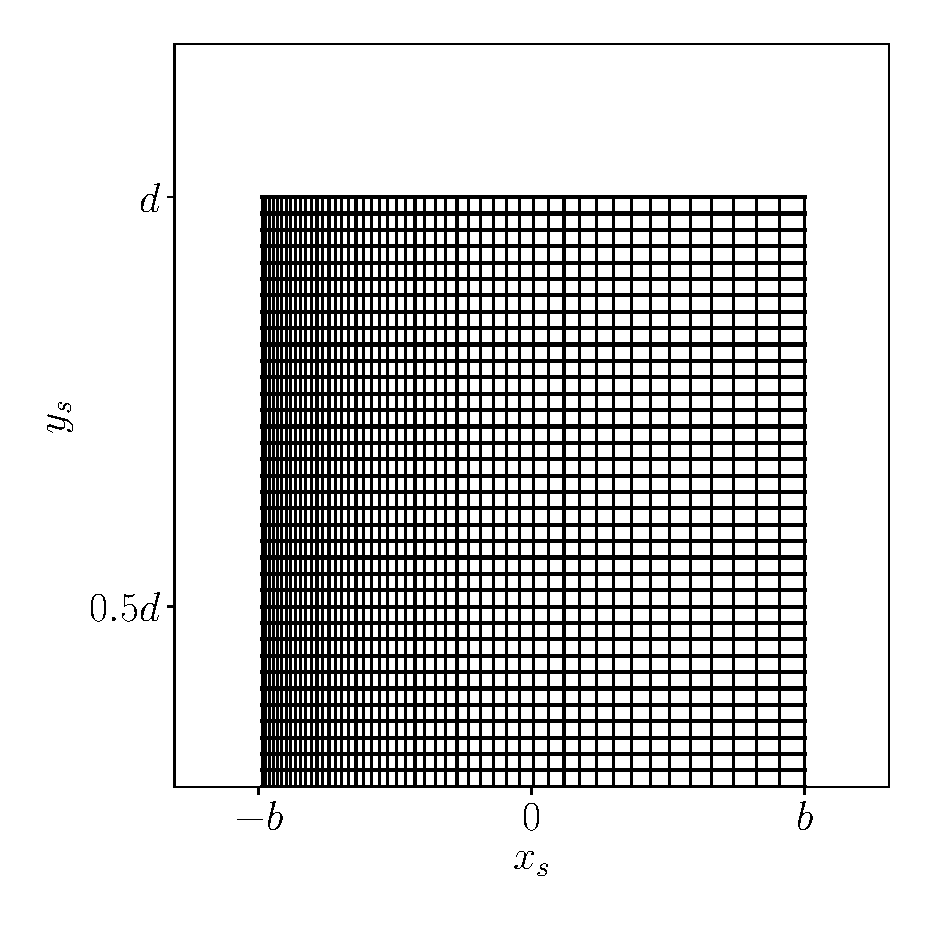
\includegraphics[width=0.6\textwidth]{../figures/Aerofoil_mesh.eps}
	\caption{Exemplo de discretização da superfície do aerofólio próximo à ponta da envergadura, com $N_y=101$ pontos distribuidos uniformemente ao longo da envergadura, e $N_x = 50$ pontos distribuidos não uniformemente ao longo da corda.}
	\label{fig:aerofoil_mesh}
\end{figure}


\subsubsection{Calculando variáveis secundárias}

Após carregar as variáveis a partir dos arquivos de texto, as funções \verb|AmT.loadTestSetup| e \verb|AmT.loadAirfoilGeom| calculam algumas variáveis secundárias e armazena-as como atributos dos objetos criados. Estas variáveis secundárias são:

\begin{itemize}
	\item Função \verb|AmT.loadTestSetup|:
	
	\begin{itemize}
		\item \verb|Mach|: número Mach $M_x = U_x/c_0$;
		\item \verb|beta|: parâmetro de Prandtl-Glauert $\beta = \sqrt{1-M_x^2}$;
		\item \verb|flow_param = (flow_dir, Mach)|: tupla de parâmetros do escoamento, onde \verb|flow_dir| é um caractere único indicando a direção do escoamento, e \verb|flow_dir = 'x'| por definição;
		\item \verb|dipole_axis|: caractere único indicando a direção do eixo dos dipolos acústicos, e \verb|dipole_axis = 'z'| por definição.
	\end{itemize}
	
	\item Função \verb|AmT.loadAirfoilGeom|:
	\begin{itemize}
		\item \verb|XYZ_airfoil|: array \verb|numpy| de dimensões $(3, N_x, N_y)$ contendo as coordenadas de cada amostra na superfície do aerofólio;
		\item \verb|dx|: array \verb|numpy| de dimensões $(N_x,)$ contendo os intervalos de amostragem (não-uniforme) da corda;
		\item \verb|dy|: intervalo de amostragem (uniforme) da envergadura.
	\end{itemize}
\end{itemize}

Estes cálculos são realizados internamente, e o usuário geralmente não precisa se preocupar com eles.

\subsubsection{Inserindo variáveis experimentais -- método alternativo}

Alternativamente, estas funções podem ser chamadas sem nenhum argumento de entrada; os objetos resultantes conterão as configurações do teste ``DARP2016'' por padrão, e estes podem ser modificados posteriormente dentro do script. Um exemplo deste método alternativo encontra-se na Listagem \ref{lst:AltLoadingVars}, onde três variáveis são modificadas e recebem novos valores. Note, porém, que é necessário executar os métodos internos \verb|MyTestSetup._calc_secondary_vars()| e \verb|MyAirfoil._calc_grid()| para recalcular as variáveis secundárias depois das variáveis primárias serem redefinidas.

\begin{lstlisting}[caption={Método alternativo para carregar variáveis},label={lst:AltLoadingVars}]
import amiet_tools as AmT

# Inicializando os objetos para armazenar variaveis
MyTestSetup = AmT.loadTestSetup()
MyAirfoil = AmT.loadAirfoilGeom()

# Redefinindo valores
MyTestSetup.Ux = 120
MyTestSetup.turb_intensity = 0.05
MyAirfoil.b = 0.15

# IMPORTANTE: recalcular as variaveis secundarias em ambos os objetos
MyTestSetup._calc_secondary_vars()
MyAirfoil._calc_grid()
\end{lstlisting}

Desta forma, as diversas variáveis relacionadas ao setup experimental e ao aerofólio utilizado podem ser importadas e combinadas; por exemplo, pode-se simular dois aerofólios diferentes dentro das mesmas condições experimentais. 


\subsubsection{Acessando as variáveis experimentais}

As variáveis lidas dos arquivos de texto podem agora ser acessadas como atributos dos objetos criados: por exemplo, usa-se o comando \verb|DARP2016Setup.c0| para acessar a velocidade do som $c_0$ contida neste objeto. As variáveis também podem ser exportadas diretamente para o ``namespace'' atual utilizando o método \verb|export_values| (pertencente às duas classes), conforme indicado na Listagem \ref{lst:ExportingVars}. Desta forma, as variáveis agora existem tanto como atributos dos objetos criados quanto como variáveis independentes dentro do namespace atual, facilitando certos cálculos e testes iterativos.

\begin{lstlisting}[caption={Exportando as variáveis para o ``namespace'' atual},label={lst:ExportingVars}]
# exportando variaveis para o namespace atual
(c0, rho0, p_ref, Ux, turb_intensity, length_scale, z_sl, Mach, beta,
flow_param, dipole_axis) = DARP2016Setup.export_values()

(b, d, Nx, Ny, XYZ_airfoil, dx, dy) = DARP2016Airfoil.export_values()
\end{lstlisting}

\subsubsection{Definindo as variáveis temporais}

As variáveis relacionadas à frequência temporal $f$ (em Hz) são criadas dentro do próprio código, dependendo do interesse do usuário. Como exemplo, vamos definir uma única frequência $f_0$ a partir da frequência não dimensional normalizada pela corda $k_0 c = 5$. Para tal, definimos o valor desejado de $f_0$ (a partir da frequência não dimensional $k_0 c$), e passamos esta variável e o objeto \verb|DARP2016TestSetup| como argumentos para a função \verb|AmT.FrequencyVars|, resultando no objeto aqui chamado \verb|FreqVars|. Este objeto é uma instância da classe \verb|FrequencyVariables|, definida no pacote \AmT{}; mais informações sobre as classes usadas no pacote \AmT{} podem ser encontradas na Seção \ref{sec:ClassDescription}. 

\begin{lstlisting}[caption={Criando variáveis relacionadas à frequência},label={lst:FrequencyVars}]
# frequency of operation
kc = 5                          # chordwise normalised frequency = k0*(2*b)
f0 = kc*c0/(2*np.pi*(2*b))      # approx 1.8 kHz

FreqVars = AmT.FrequencyVars(f0, DARP2016Setup)
(k0, Kx, Ky_crit) = FreqVars.export_values()
\end{lstlisting}

Similarmente, os valores aqui calculados podem ser acessados como atributos do objeto \verb|FreqVars|, ou exportados para o namespace atual através do método \verb|FreqVars.export_values|. Esta função também calcula as seguintes variáveis secundárias para uma dada frequência $f0$:

\begin{itemize}
	\item \verb|k0|: número de onda acústico $k_0$ [rad/m];
	\item \verb|Kx|: número de onda longitudinal da rajada $\kappa_\chi = \omega/U_x$;
	\item \verb|Ky_crit|: número de onda crítico lateral de rajada $k_\psi^{crit}$.
\end{itemize}

Para cálculos envolvendo múltiplas frequências, recomenda-se realizar um loop sobre as frequências de interesse, e recriar o objeto \verb|FreqVars| ao início de cada iteração.

% *-*-*-*-*-*-*-*-*-*-*-*-*-*-*-*-*-*-*-*-*-*-*-*-*-*-*-*-*-*-*-*-*-*-*-*-*-*-
\newpage
\section{Exemplos}
\label{sec:Examples}

Esta Seção irá descrever alguns aspectos dos scripts de teste contidos dentro do diretório \verb|test_scripts|, armazenados na página do projeto \AmT{} no GitHub. Este tutorial descreverá o uso das funções contidas no pacote \AmT{} e seus resultados, mas não descreverá em detalhes outras partes dos códigos, tais como comandos usados para plotar uma figura.

\subsection{Exemplo 1: Interação de Rajada Única}
\label{sec:SingleGustInteraction}

Como primeiro exemplo, vamos usar o pacote \AmT{} para calcular a distribuição do ``salto'' de pressão $\Delta p(x_s, y_s)$ na superfície do aerofólio em resposta a uma única rajada turbulenta em uma única frequência, e as funções de diretividade do campo acústico nas direções da corda e da envergadura. Este exemplo corresponde ao script de teste \verb|TestScript1_SingleGustPlots.py|.

A primeira parte do script está apresentada na Listagem \ref{lst:TestScript1_1stPart}. Primeiramente, seguimos as instruções descritas na Seção \ref{Sec:UsingThePackage} para importar os pacotes \verb|numpy|, \verb|amiet_tools| e \verb|matplotlib|, e carregar as variáveis experimentais a partir dos arquivos de texto \verb|DARP2016_TestSetup.txt| e \verb|DARP2016_AirfoilGeom.txt|. Após carregar as variáveis, estas são exportadas para o ``namespace'' atual. 

\begin{lstlisting}[caption={Script de teste 1 - início},label={lst:TestScript1_1stPart}]
import numpy as np
import amiet_tools as AmT

import matplotlib.pyplot as plt

# %% *-*-*-*-*-*-*-*-*-*-*-*-*-*-*-*-*-*-*-*-*-*-*-*-*-*-*-*-*-*-*-*-*-*-*-*-*-
# carrega as condicoes do experimento a partir de um arquivo de texto
DARP2016Setup = AmT.loadTestSetup('DARP2016_TestSetup.txt')

# exportar variaveis para o namespace atual
(c0, rho0, p_ref, Ux, turb_intensity, length_scale, z_sl, Mach, beta,
flow_param, dipole_axis) = DARP2016Setup.export_values()

# %% *-*-*-*-*-*-*-*-*-*-*-*-*-*-*-*-*-*-*-*-*-*-*-*-*-*-*-*-*-*-*-*-*-*-*-*-*-
# carrega a geometria do aerofolio a partir de um arquivo de texto
DARP2016Airfoil = AmT.loadAirfoilGeom('DARP2016_AirfoilGeom.txt')

(b, d, Nx, Ny, XYZ_airfoil, dx, dy) = DARP2016Airfoil.export_values()
XYZ_airfoil_calc = XYZ_airfoil.reshape(3, Nx*Ny)
\end{lstlisting}

Aqui também realizamos um passo importante para os cálculos numéricos: redimensionamos o array \verb|XYZ_airfoil| de coordenadas na superfície do aerofólio para criarmos um array \verb|XYZ_airfoil_calc| de dimensões $(3, N_x N_y)$, que será útil para a realização de alguns cálculos posteriormente.

Em seguida, definimos a frequência temporal de interesse, conforme indicado na Listagem \ref{lst:TestScript1_frequency}. Para este exemplo, iniciamos o cálculo com um valor de frequência não dimensional normalizada pela corda $k_0 c = 5$, o que resulta em uma frequência temporal $f \approx 1.8$ kHz. Por conveniência, exportamos as variáveis mais uma vez para o ``namespace'' atual.

\begin{lstlisting}[caption={Script de teste 1 - definindo a frequência},label={lst:TestScript1_frequency}]
# frequencia de operacao
kc = 5                          # freq normalizada pela corda = k0*(2*b)
f0 = kc*c0/(2*np.pi*(2*b))      # approx 1.8 kHz

FreqVars = AmT.FrequencyVars(f0, DARP2016Setup)
(k0, Kx, Ky_crit) = FreqVars.export_values()
\end{lstlisting}

Para fins ilustrativos, escolhemos uma amplitude de rajada $\hat{w}_0=1$. Em seguida, escolhemos um valor para o número de onda lateral de rajada $k_\psi$ (aqui escolhemos $k_\psi = 0.35 k_\psi^{crit}$ para fins ilustrativos), e calculamos a flutuação de pressão $\Delta p$ sobre o aerofólio em resposta a esta rajada usando a função \verb|AmT.delta_p|, conforme indicado na Listagem \ref{lst:TestScript1_deltaP}. O resultado é armazenada na variável \verb|delta_p1|, um array \verb|numpy| de dimensões $(\verb|Ny|, \verb|Nx|)$ contendo os valores do salto de pressão $\Delta p$ em cada ponto na superfície do aerofólio. Note que, como a função $\Delta p$ não depende da altura do aerofólio $z_s$, passamos apenas as primeiras duas coordenadas ($x_s$ e $y_s$) do array \verb|XYZ_airfoil| como argumento para a função \verb|AmT.delta_p|.

Ainda na Listagem \ref{lst:TestScript1_deltaP}, realizamos mais um passo importante para os cálculos numéricos: redimensionamos o array \verb|delta_p1| para criar um array \verb|delta_p1_calc| de dimensão $(N_x N_y,)$, e multiplicamos este array pelos intervalos de amostragem \verb|dx| (um array) e \verb|dy| (um número). Desta forma, cada elemento do array redimensionado \verb|delta_p1_calc| conterá o valor da flutuação de pressão $\Delta p$ calculada para o elemento localizado em $(x_s, y_s)$, e ponderada pela área do elemento $\ud x_s \ud y_s$ .

\begin{lstlisting}[caption={Script de teste 1 - calculando o salto de pressão},label={lst:TestScript1_deltaP}]
# amplitude da rajada
w0 = 1

# numero de onda lateral da rajada
ky = 0.35*ky_crit

# Calcula o salto de pressao sobre o aerofolio
delta_p1 = AmT.delta_p(rho0, b, w0, Ux, Kx, ky, XYZ_airfoil[0:2], Mach)

# redimensiona o array de salto de pressao, aplica pesos por area da amostragem
delta_p1_calc = (delta_p1*dx).reshape(Nx*Ny)*dy
\end{lstlisting}

A Figura \ref{fig:DeltaP_Kphi_035} mostra a parte real $\textrm{Re}\{\Delta p \}$ e a magnitude $|\Delta p|$ (em decibéis) do salto de pressão (normalizado) $\Delta p$ obtido com os comandos listados acima. Note como a flutuação de pressão apresenta maior magnitude próximo ao bordo de ataque, e tende a zero no bordo de fuga. Note ainda a oscilação na direção lateral, devido ao número de onda lateral da rajada $k_\psi \neq 0$.

\begin{figure}[htbp]
	\centering
	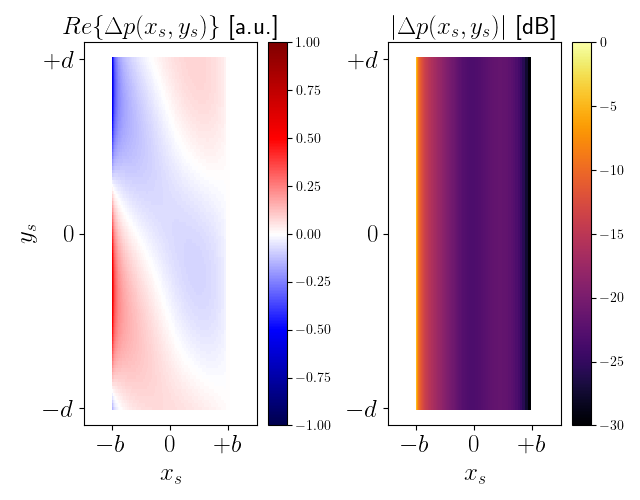
\includegraphics[width=0.65\textwidth]{../figures/DeltaP_Kphi_035.png}
	\caption{Parte real $\textrm{Re}(\Delta p)$ e a magnitude $|\Delta p|$ (em decibéis) do salto de pressão (normalizado) $\Delta p$ obtido com $k_\psi=0.35k_\psi^{crit}$.}
	\label{fig:DeltaP_Kphi_035}
\end{figure}

Em seguida, calculamos as funções de diretividade do campo acústico nas direções da corda (plano $y=0$) e da envergadura (plano $x=0$). Para isso, criamos uma série de pontos a uma distância \verb|R_farfield| do centro do aerofólio, arranjados de forma semicircular, com espaçamento angular uniforme, e calculamos o campo acústico visto por esses observadores. Estes comandos estão indicados na Listagem \ref{lst:TestScript1_farFieldObs}, onde usamos $M=181$ observadores em cada direção, e os arrays resultantes \verb|XZ_farfield| e \verb|YZ_farfield| possuem dimensões $(3, M)$.

Dadas os arrays \verb|XZ_farfield| e \verb|YZ_farfield| de coordenadas dos observadores distantes nas direções da corda e da envergadura, respectivamente, calculamos a matriz de funções de transferência para cada par fonte-observador através da função \verb|AmT.dipole3D|. As matrizes resultantes \verb|G_ffXZ| e \verb|G_ffYZ| são arrays \verb|numpy| de dimensões $(M, N_x N_y)$.

A pressão acústica $p$ vista por cada observador é então calculada através do produto matricial \verb|G_ffXZ @ delta_p1_calc|, onde o símbolo \verb|@| é usado no pacote \verb|numpy| para indicar produto escalar entre dois arrays. Note que como a variável \verb|delta_p1_calc| já inclui uma ponderação pela área de cada elemento $\ud x_s \ud y_s$ da superfície do aerofólio, a operação aqui descrita pode ser entendida como o cálculo numérico da integral de superfície definida na Eq. \ref{eq:ac_radiation_single_gust}:

\begin{IEEEeqnarray}{rCl}
	p(\mathbf{r}, \omega) & = & \int_{-d}^{+d} \int_{-b}^{+b} \Delta p(\mathbf{r}_s, \omega) \frac{\partial }{\partial z_s} G_{U_x}(\mathbf{r} | \mathbf{r}_s, \omega) \ud x_s \ud y_s \nonumber \\
		& \approx & \sum_{N_x} \sum_{N_y} \frac{\partial }{\partial z_s} G_{U_x}(\mathbf{r} | \mathbf{r}_s, \omega) \ \left[ \Delta p(\mathbf{r}_s, \omega) \ud x_s \ud y_s \right].
\end{IEEEeqnarray}


\begin{lstlisting}[caption={Script de teste 1 - observadores no campo distante},label={lst:TestScript1_farFieldObs}]
# Cria 181 observadores no campo distante
R_farfield = 50     # [m]
theta_farfield = np.linspace(-np.pi/2, np.pi/2, 181)
xy_farfield = R_farfield*np.sin(theta_farfield)
z_farfield = -R_farfield*np.cos(theta_farfield)

XZ_farfield = np.array([xy_farfield, np.zeros(xy_farfield.shape), z_farfield])
YZ_farfield = np.array([np.zeros(xy_farfield.shape), xy_farfield, z_farfield])

# Campo acustico gerado pelo aerofolio nos observadores
p_XZ_farfield = np.zeros(x_farfield.shape, 'complex')
p_YZ_farfield = np.zeros(x_farfield.shape, 'complex')

# *-*-*-*-*-*-*-*-*-*-*-*-*-*-*-*-*-*-*-*-*-*-*-*-*-*-*-*-*-*-*-*-*-*-*-*-*-
# Calcula matrizes de funcao de transferencia para dipolos com conveccao entre
# cada fonte e cada observador
G_ffXZ = AmT.dipole3D(XYZ_airfoil_calc, XZ_farfield, k0, dipole_axis,
flow_param)

G_ffYZ = AmT.dipole3D(XYZ_airfoil_calc, YZ_farfield, k0, dipole_axis,
flow_param)

# Calcula a pressao acustica no campo distante
p_XZ_farfield = G_ffXZ @ delta_p1_calc
p_YZ_farfield = G_ffYZ @ delta_p1_calc
\end{lstlisting}

As funções de diretividade da radiação acústica nas direções da corda e da envergadura estão demonstradas na Figura \ref{fig:dir_XZ_YZ_Kphi_035}. Note o caráter ``inclinado'' da diretividade na direção da envergadura, característica típica da radiação em resposta a rajadas com $k_\psi \neq 0$.

\begin{figure}
	\centering
	\subfloat[]{
		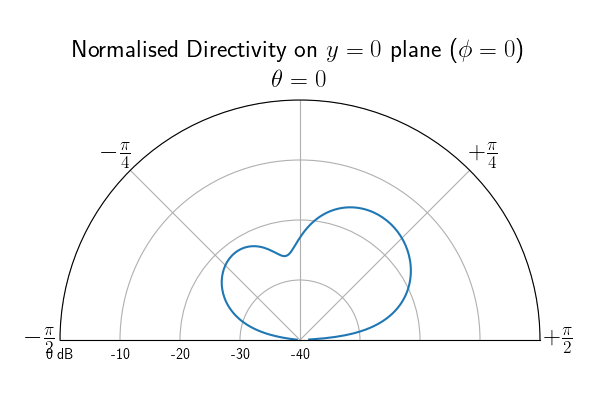
\includegraphics[width=0.5\textwidth]{../figures/dir_XZ_Kphi_035.png}
		\label{fig:dir_XZ_Kphi_035}
	}
	\subfloat[]{
		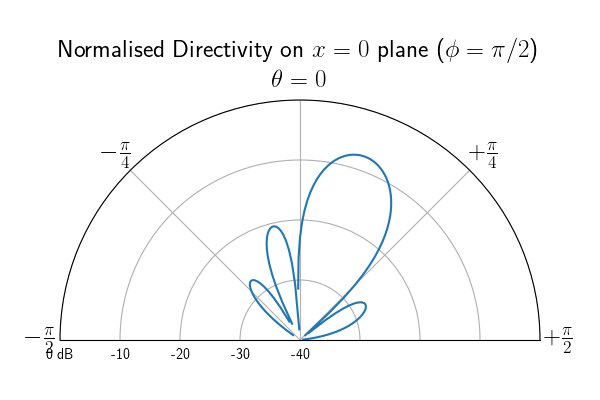
\includegraphics[width=0.5\textwidth]{../figures/dir_YZ_Kphi_035.png}
		\label{fig:dir_YZ_Kphi_035}
	}
	\caption{Funções de diretividade da radiação acústica em resposta a uma rajada única, com $k_0 c = 5$, $M_x \approx 0.17$. \protect\subref{fig:dir_XZ_Kphi_035} diretividade na direção da corda; \protect\subref{fig:dir_YZ_Kphi_035} diretividade na direção da envergadura.}
	\label{fig:dir_XZ_YZ_Kphi_035}
\end{figure}



% *-*-*-*-*-*-*-*-*-*-*-*-*-*-*-*-*-*-*-*-*-*-*-*-*-*-*-*-*-*-*-*-*-*-*-*-*-*-
\clearpage
\newpage
\section{Pseudocódigo}

O pseudocódigo usado para calcular o espectro cruzado $S_{\Delta p \Delta p'}$ da pressão de superfície do aerofólio e/ou o espectro cruzado $S_{pp'}$ do ruído radiado é mostrado abaixo, retirado de \cite{Casagrande_etal2020}. A maior parte das instruções mostradas abaixo possuem funções Python equivalentes ou métodos associados no pacote \AmT{}, e não precisam ser implementadas pelo usuário final. Para mais detalhes sobre o uso destas funções, veja a documentação e os scripts de exemplo no pacote.

\begin{algorithm}
	\caption{Pseudocódigo para o modelo de predição de ruído de interação turbulência-aerofólio do pacote \texttt{amiet\_tools}}
	\label{alg:amiet_pseudocode}
	\begin{algorithmic}[1] % Define line numbers
		\State Definir as variáveis do ambiente de teste: $c_0, \rho_0, p_{ref}, U_x, \overline{w^2}, \Lambda, z_{sl}, M_x, \beta$
		\State Definir as variáveis da geometria do aerofólio: $b, d, N_x, N_y, \Delta x_s, \Delta y_s$
		\State Calcular a amostragem da corda do aerofólio $x_s[n], \ n \in [1, \ldots, N_x]$
		\State Calcular a amostragem da envergadura do aerofólio $y_s[n], \ n \in [1, \ldots, N_y]$
		\State Definir as coordenadas dos observadores $\mathbf{r}_m = (x_m, y_m, z_m), \ m \in [1, \ldots, M]$
		
		\If{usando correção de camada cisalhante}
		\ForAll{pares $(m, n)$ de pontos observador-aerofólio $(\mathbf{r}_m|\mathbf{r}_s)$}
		\State Calcular os pontos de cruzamento da camada cisalhante $\mathbf{r}_l(m, n)$ e tempos de propagação $\tau_{sm}(m, n)$
		\EndFor
		\EndIf
		
		\For{cada frequência $f \in [f_{min}, \ldots, f_{max}]$}
		\State Calcular $k_0, \kappa_\chi, k_\psi^{crit}$
		\State Calcular valores de números de onda de rajada $k_\psi \in [-k_\psi^{max}, k_\psi^{max}]$
		\State Calcular intervalo de amostragem dos números de onda de rajada $\Delta k_\psi$
		\State Calcular espectro de energia dos números de onda de rajada $\Phi_{ww}(k_\psi)$
		\State Calcular matriz $\partial G(\mathbf{r}_m|\mathbf{r}_s)/\partial z_s$ para todos os pares $(m, n)$ de pontos observador-aerofólio; 
		\State Inicializar $S_{\Delta p \Delta p'} \gets 0$
		\State Inicializar $S_{p p'} \gets 0$
		\For{cada rajada $k_\psi \in [-k_\psi^{max}, k_\psi^{max}]$}
		\State $w(k_\psi) \gets \sqrt{\Phi_{ww}(k_\psi)}$
		\State Calcular $\Delta p(x_s, y_s, k_\psi)$ usando $w(k_\psi)$ 
		\State $S_{\Delta p \Delta p'}(\mathbf{r}_s, \mathbf{r}_s') \gets S_{\Delta p \Delta p'}(\mathbf{r}_s, \mathbf{r}_s') + \left[ \Delta p(x_s, y_s, k_\psi) \cdot \Delta p^*(x_s', y_s', k_\psi) \right] \cdot U_x \cdot \Delta k_\psi$ \label{alg:crossproduct}
		\EndFor
		\State $S_{pp'}(\mathbf{r}_m, \mathbf{r}_{m'}) \gets 4 \pi \left[ S_{\Delta p \Delta p'} \cdot (\Delta x_s \cdot \Delta y_s) \cdot (\Delta x_s' \cdot \Delta y_s') \right] \cdot \left[ \partial G(\mathbf{r}_m|\mathbf{r}_s)/\partial z_s \right] \cdot \left[ \partial G(\mathbf{r}_{m'}|\mathbf{r}_s')/\partial z_s \right]$
		\EndFor
	\end{algorithmic}
\end{algorithm}

\clearpage
\newpage

% *-*-*-*-*-*-*-*-*-*-*-*-*-*-*-*-*-*-*-*-*-*-*-*-*-*-*-*-*-*-*-*-*-*-*-*-*-*-
\section{Descrição das classes}
\label{sec:ClassDescription}

O pacote \verb|amiet_tools| utiliza classes --- i.e. estruturas de abstração usadas em programação orientada a objetos --- para armazenar dados relacionados aos diferentes aspectos da simulação. As três classes utilizadas em\AmT{} estão descritas abaixo, seguidas de uma lista de seus atributos:

\begin{itemize}
	\item Classe \verb|TestSetup|:
	\begin{itemize}
		\item \verb|TestSetup.c0|: velocidade do som em um meio em repouso $c_0$ (em m/s);
		\item \verb|TestSetup.rho0|: densidade do ar $\rho_0$ (em kg/m$^3$);
		\item \verb|TestSetup.p_ref|: pressão acústica de referência $p_{ref} = 20 \mu$Pa RMS;
		\item \verb|TestSetup.Ux|: velocidade média do escoamento $U_x$ (em m/s);
		\item \verb|TestSetup.turb_intensity|: intensidade da turbulência $\sqrt{\overline{w^2}}/U_x$;
		\item \verb|TestSetup.length_scale|: escala de comprimento de turbulência $\Lambda$ (em m);
		\item \verb|TestSetup.z_sl|: altura da camada cisalhante $z_{sl}$ (em m);
		\item \verb|TestSetup.flow_dir|: caractere único indicando a direção do escoamento (i.e. \verb|'x'| para indicar escoamento na direção $+x$);
		\item \verb|TestSetup.dipole_axis|: caractere único indicando a direção do eixo dos dipolos (i.e. `\verb|z|' para dipolos apontando ``para cima'', na direção $+z$);
		\item \verb|TestSetup.Mach|: número de Mach do escoamento $M_x = U_x/c_0$;
		\item \verb|TestSetup.beta|: fator de Prandtl-Glauert $\beta = \sqrt{1-M_x^2}$.
	\end{itemize}
	
	\item Classe \verb|AirfoilGeom|:
	\begin{itemize}
		\item \verb|AirfoilGeom.b|: semi corda do aerofólio $b = c/2$ (em m);
		\item \verb|AirfoilGeom.d|: semi envergadura do aerofólio $d = L/2$ (em m);
		\item \verb|AirfoilGeom.Nx|: número de amostras sobre a corda $N_x$, amostragem não-uniforme;
		\item \verb|AirfoilGeom.Ny|: número de amostras sobre a envergadura $N_y$, amostragem uniforme;
		\item \verb|AirfoilGeom.dx|: intervalos de amostragem sobre a corda $\Delta x_s$  (calculado internamente)
		\item \verb|AirfoilGeom.dy|: intervalo de amostragem sobre a envergadura $\Delta y_s$  (calculado internamente).
	\end{itemize}
	
	\item Classe \verb|FrequencyVariables|:
	\begin{itemize}
		\item \verb|FrequencyVariables.freq|: frequência $f$ (em Hz);
		\item \verb|FrequencyVariables.k0|: número de onda acústico $k_0 = 2 \pi f/c_0$;
		\item \verb|FrequencyVariables.Kx|: número de onda de rajada na direção da corda $\kappa_\chi = \omega/U_x$;
		\item \verb|FrequencyVariables.Ky_crit|: número de onda crítico de rajada na direção da envergadura $k_\psi^{crit}$.
	\end{itemize}
\end{itemize}

Uma instância de cada classe é criada para armazenar os valores das variáveis relacionados às condições de um experimento e para passá-las às diferentes funções no pacote. Valores numéricos podem ser atribuídos diretamente através de um script em Python, ou podem ser lidos em um arquivo externo através das funções \verb|loadTestSetup| e \verb|loadAirfoilGeom|. 

Uma quarta classe chamada \verb|MicArrayCsmHDF5| também está inclusa no pacote, e permite a leitura e escrita de dados de CSM de arranjos de microfones no formato HDF5 adotado pela comunidade ``Array Methods'' \cite{Bahr_etal2017, Sarradj_etal2017} para compartilhar dados de ``beamforming''.

% *-*-*-*-*-*-*-*-*-*-*-*-*-*-*-*-*-*-*-*-*-*-*-*-*-*-*-*-*-*-*-*-*-*-
\clearpage
\newpage
\label{Bibliography}
\bibliographystyle{unsrtnat} 
\bibliography{../Bibliography} 
\end{document}
